%%%%%%%%%%%%%%%%%%%%%%%%%%%%%%%%%%%%%%%%%
% Beamer Presentation
% LaTeX Template
% Version 1.0 (10/11/12)
%
% This template has been downloaded from:
% http://www.LaTeXTemplates.com
%
% License:
% CC BY-NC-SA 3.0 (http://creativecommons.org/licenses/by-nc-sa/3.0/)
%
%%%%%%%%%%%%%%%%%%%%%%%%%%%%%%%%%%%%%%%%%

%----------------------------------------------------------------------------------------
%	PACKAGES AND THEMES
%----------------------------------------------------------------------------------------

\documentclass[usenames,dvipsnames,table]{beamer}

\mode<presentation> {

\usetheme{Madrid}
%\setbeamertemplate{footline} % To remove the footer line in all slides uncomment this line
%\setbeamertemplate{footline}[page number] % To replace the footer line in all slides with a simple slide count uncomment this line
\setbeamertemplate{navigation symbols}{} % To remove the navigation symbols from the bottom of all slides uncomment this line
}

\usepackage{amsmath}
\usepackage{graphicx} % Allows including images
\usepackage{booktabs} % Allows the use of \toprule, \midrule and \bottomrule in tables
\usepackage{listings}
\usepackage{xcolor}
\usepackage{xfrac}
% \usepackage{enumitem}

%----------------------------------------------------------------------------------------
%	TITLE PAGE
%----------------------------------------------------------------------------------------

\title[ABDA Ch 5]{Applied Bayesian Data Analysis --- Chapter 5}

\author{Kim Albertsson} % Your name
\institute[LTU and CERN]
{
CERN and Luleå University of Technology \\
\medskip
\textit{kim.albertsson@ltu.se}
}
\date{\today}

\newcommand{\cgy}{\cellcolor{gray!25}}
\newcommand{\cgr}{\cellcolor{green!25}}
\newcommand{\cye}{\cellcolor{orange!25}}
\newcommand{\ccb}{\cellcolor{Cerulean!25}}

\begin{document}

\begin{frame}
\titlepage % Print the title page as the first slide
\end{frame}

% \begin{frame}
% \frametitle{}
% \begin{itemize}
% \item
% \end{itemize}
% \end{frame}

%----------------------------------------------------------------------------------------
%	PRESENTATION SLIDES
%----------------------------------------------------------------------------------------
\section{Chapter 5}
\begin{frame}
\begin{center}
{\huge{Chapter 5}}
\\\vspace{2em}
Gaining intuition about Bayes' rule
\vspace{5em}
\end{center}
\end{frame}


\begin{frame}
\frametitle{Introduction}
Bayes' rule is a \emph{central} concept of Bayesian statistics

\begin{align*}
p(c\vert r) &= \frac{p(r\vert c) p(c)}{p(r)} \tag{5.5}
\end{align*}

One primary usecase: Estimate probability of model paramters given data.

\end{frame}



\begin{frame}
\frametitle{Derivation of Bayes' Rule}

\begin{align*}
p(c\vert r) &= \frac{p(r, c)}{p(r)} \tag{5.1} \\
p(r, c) &= p(c\vert r) p(r) \tag{5.2} \\
p(r, c) &= p(r\vert c) p(c) \tag{5.3} \\
p(c\vert r) p(r) &= p(r\vert c) p(c) \tag{5.4}
\end{align*}

Bayes' Rule:
\begin{align*}
p(c\vert r) &= \frac{p(r\vert c) p(c)}{p(r)} \tag{5.5}
\end{align*}

Remember that:
\begin{align*}
p(R=r) &= \int p(R=r, C=c)\, dc \\
p(C=c\vert R=r) &= \frac{p(R=r\vert C=c) p(C=c)}{\int p(R=r, C=c')\, dc'}
\end{align*}

\end{frame}


\begin{frame}
\frametitle{A Note on Notation}
Given a probability distribution $p(r, c)$, what does $p(0.5)$ signify?

\vspace{1em}
Unclear!

\vspace{1em}
More clear alternatives: $p_r(0.5)$ or $p(R=0.5)$

\vspace{1em}
Mathematically there is no problem with: $p(R=c, C=r)$.

Keep track of you variables and observables!

\end{frame}

\begin{frame}
\frametitle{Bayes' rule intuited from a two-way discrete table}

\begin{align*}
p(c\vert r)  &= \frac{p(r\vert c) p(c)}{p(r)} \tag{5.5} \\
p(\mathrm{E}= \mathrm{Blue}|\mathrm{H}=\mathrm{Red}\})
&= \frac{\textcolor{green}{p(\mathrm{H}=\mathrm{Red}\}
                             |\textcolor{green}{\mathrm{E}=\mathrm{Blue}})
                             p(\mathrm{E}=\mathrm{Blue})}}
       {\textcolor{orange}{p(\mathrm{H}=\mathrm{Red})}}
\end{align*}

\textbf{Joint probabilities}
\begin{table}
\begin{tabular}{lccccc}
           & Black & Brown & Red  & Blond & $\sum$ \\
     Brown &\cgy0.11&\cgy0.20&\cye0.04&\cgy0.01& 0.37 \\
      Blue &\cgy0.03&\cgy0.14&\cgr0.03&\cgy0.16& 0.36 \\
     Hazel &\cgy0.03&\cgy0.09&\cye0.02&\cgy0.02& 0.16 \\
     Green &\cgy0.01&\cgy0.05&\cye0.02&\cgy0.03& 0.11 \\
    $\sum$ &  0.18 &  0.48 & 0.12 &  0.21 & 1.0   \\
\end{tabular}
\end{table}
\end{frame}

\begin{frame}
\frametitle{Example: Test for Disease}

Diagnosis of rare disease.

Suppose one in a thousand has it. $\implies p(\theta=\ddot\frown) = 0.001$
Suppose test with true postitive rate 0.99 $\implies p(T=+\vert \theta=\ddot\frown) = 0.99$
Suppose also false postitive rate 0.05 $\implies p(T=+\vert \theta=\ddot\smile) = 0.05$

\vspace{1em}
Question: Given a postitive test, what is the probability that the subject is ill?

\begin{align*}
p(\theta=\ddot\frown\vert T=+) &= \frac{p(T=+\vert \theta=\ddot\frown) p(\theta=\ddot\frown)}{p(T=+)}
\end{align*}

\begin{align*}
p(\theta=\ddot\smile) &= 1 - p(\theta=\ddot\frown) = 0.999 \\
p(T=+) &= p(T=+\vert \theta=\ddot\frown)p(\theta=\ddot\frown) \\
         & + p(T=+\vert \theta=\ddot\smile)p(\theta=\ddot\smile)
\end{align*}
\end{frame}




\begin{frame}
\frametitle{Applied to Parameters and Data}
Central question: Given some data, how likely are our model parameters?

\begin{align*}
p(\theta\vert X) &= \frac{p(X\vert \theta) p(\theta)}{p(X)}
\end{align*}

Close analogy to the disease example, imagine big table.

\begin{align*}
p(\theta\vert X)      &: \mathrm{posterior} \\
p(X\vert \theta)      &: \mathrm{likelihood} \\
p(\theta)             &: \mathrm{prior} \\
p(X)                  &: \mathrm{evidence} \\
\end{align*}

\end{frame}





\begin{frame}
\frametitle{Data Order Invariance}

$h$ denotes probability of heads.
$t_0t_1\ldots$ is a sequence of coin flips.

\begin{align*}
p(h|t_0t_1\ldots) &= p(h|t_0, t_1, \ldots)\\
                  &= \frac{p(t_0, t_1, \ldots|h)}{p(t_0, t_1, \ldots)}p(h) \\
                  &\mathrm{assume\ independence}\\
                  &= \frac{p(t_0|h) p(t_1|h) p(\ldots|h)}{p(t_0)p(t_1)p(\ldots)}p(h)\\
                  &= \ldots \cdot \frac{p(t_1|h)}{p(t_1)}
                            \cdot \frac{p(t_0|h)}{p(t_0)}
                            \cdot p(h)
\end{align*}

Since multiplication is commutative, the order of the data does not matter.

\end{frame}






\begin{frame}
\frametitle{Complete Example: Estimating Bias in a Coin (I)}

Likelihood for a coin flip:
\begin{align*}
p(t\vert \theta) = \theta^t(1-\theta)^{1-t}; t \in {0, 1}\ \mathrm{Bernoulli\ distribution}
\end{align*}

For several flips:
\begin{align*}
p(T\vert \theta)&= \prod_{t_i \in T} \theta^{t_i}(1-\theta)^{1-t_i} \\
                &= \theta^z(1-\theta)^{N-z}
\end{align*}

where $z$ is total number of heads and $N-z$ is total number of tails.

That is, the probability of heads given a \emph{propensity} for heads.

\end{frame}



\begin{frame}
\frametitle{Complete Example: Estimating Bias in a Coin (II)}
\begin{columns}[c]
\column{.5\textwidth}
Qualitatively: If we assume a coin is most probably fair

\vspace{1em}
If we measure a single flip and it is heads, this indicates we should shift our beliefs so heads is more likely.

\column{.5\textwidth}
\begin{figure}
\centering
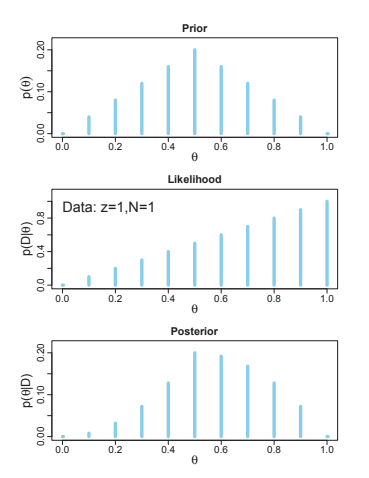
\includegraphics[width=\linewidth]{img/fig5_1}
\end{figure}
\end{columns}
\end{frame}


\begin{frame}
\frametitle{Influence of sample size on the posterior}
\begin{columns}[c]
\column{.5\textwidth}
A larger sample size makes us less reliant on the prior. Note that the prior is the same in both plots!

This will be derived analytically for specific priors and likelihoods in the next chapter.

\column{.5\textwidth}
\begin{figure}
\centering
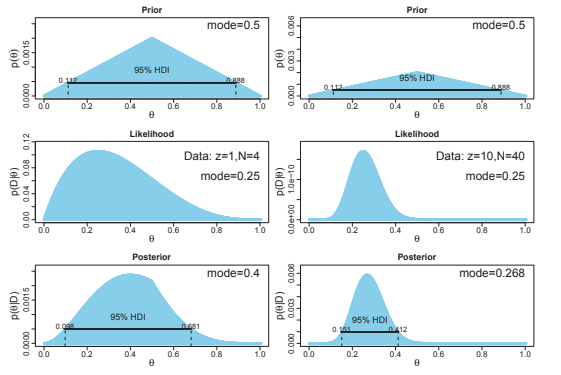
\includegraphics[width=\linewidth]{img/fig5_2}
\end{figure}
\end{columns}
\end{frame}

\begin{frame}
\frametitle{Influence of the prior on the posterior}
\begin{columns}[c]
\column{.5\textwidth}
Compare to previous plot.

The prior can be thought of (through data order invariance) as incorporating previous data. Thus a flatter prior broades the posterior, while a sharper makes it more narrow (assuming it is reasonably correct).

\column{.5\textwidth}
\begin{figure}
\centering
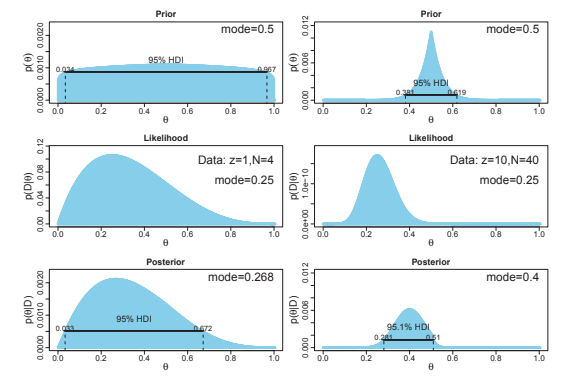
\includegraphics[width=\linewidth]{img/fig5_3}
\end{figure}
\end{columns}
\end{frame}




\begin{frame}
\frametitle{Why Bayesian Inference Can Be Difficult}

Bayes rule:
\begin{align*}
p(\theta\vert X) &= \frac{p(X\vert \theta) p(\theta)}{p(X)}
\end{align*}

\textbf{Analytic solution:} is not in general easy, or even possible. Exceptions include specific prior-likelihood combinations called conjugate priors. (A prior conjugate to the given likelihood.)

One can also approximate tricky integrals with easier to integrate functions. Called \emph{variational approximation}.

\textbf{Grid approximation:} Discretisize, and numerically solve integrals. Fine for small parameter spaces, but quickly runs into the \emph{curse of dimensionality}.

\textbf{Sampling approximation:} Randomly sample the posterior through \emph{Markov-chain Monte-Carlo} methods. These methods skip the evaluation of the integrals. Lead to Bayesian methods gaining practical use.

\end{frame}






\end{document} 